%Thus far in this work a solution to simplify and automate design the process of all digital PLL loop filter designs comprised of (1) an automated loop filter optimization and design engine, and (2) a discrete-event, time domain PLL simulator to evaluate the designed filters with full time-discretization and quantization nonlinearity effects. I
In this discussion, the performance of the presented design solution will first be evaluated with a design example. Then, a comparison of the presented solution will be made to existing solutions in literature, pointing out advantages and disadvantages of this work. Finally, a general discussion will be made covering areas of improvement, reasoning for the central design choices made, and considerations for usage the framework.

\subsection{State of art}
	\begin{figure}[htb!]
	    \centering
	    \begin{subfigure}{0.5\textwidth}
	        \centering
	        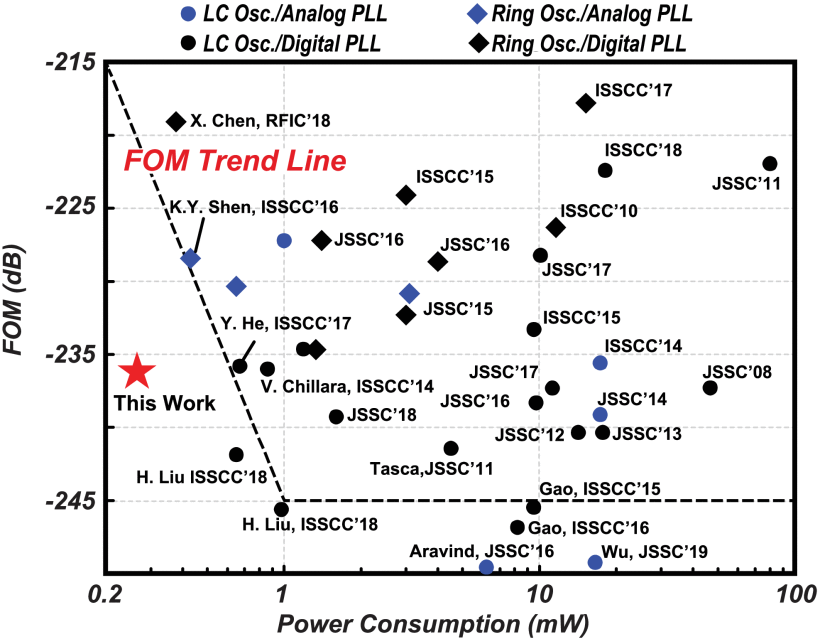
\includegraphics[width=1\textwidth, angle=0]{./figs/liu24-fom}
	    \end{subfigure}%
	    \begin{subfigure}{0.5\textwidth}
	        \centering
	        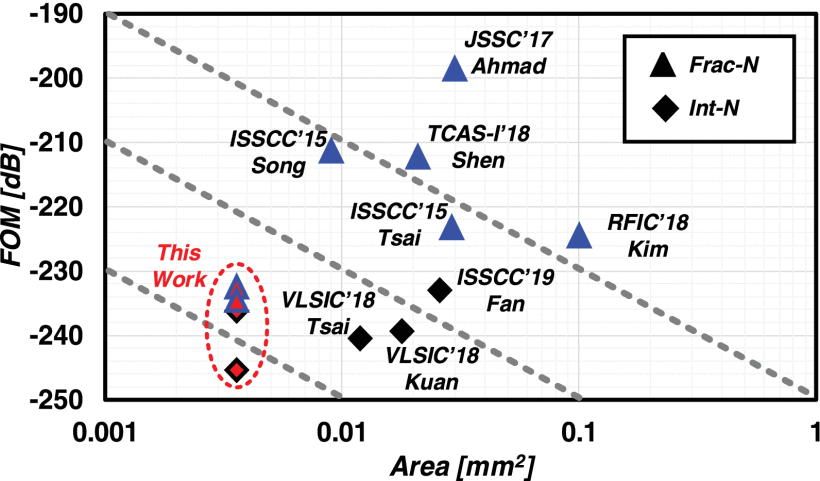
\includegraphics[width=1\textwidth, angle=0]{./figs/liu_5nm}
	    \end{subfigure}
	    % \caption{Approximate model for ring oscillator inverter delay cell.}
	\end{figure}



\pagebreak
\subsubsection{Results Comparison of Design Approaches}
A comparison of the two design approaches shows that the PLL utilizing the gear switching results in a superior result using the design automation framework of this work. The usage of gear switching results in lower phase noise than approach 1, with total phase noise power (residual phase modulation) of 4.36$\times 10^{-2}$ rad$^2$ versus 3.37$\times 10^{-1}$ rad$^2$. Additionally, the lock time is significantly lower in the PLL with gear switching, at an average of 5.96 $\mu$s versus 19.32 $\mu$s. Therefore it has been shown that this framework offers the capability to design gear-switching PLLs with performance advantages to static loop filter PLL designs.

	% \begin{figure}[htb!]
	% 	\center\includegraphics[width=1.0\textwidth, angle=0]{figs/x.pdf}
	% 	\caption{Transient simulation of optimal design.}
	% 	\label{fig:des_ex_trans}
	% \end{figure}
	% \FloatBarrier

	% \begin{figure}[htb!]
	% 	\center\includegraphics[width=1.0\textwidth, angle=0]{figs/x.pdf}
	% 	\caption{Variation Simulation for KDCO.}
	% 	\label{fig:var_lock}
	% \end{figure}
	% \FloatBarrier

	% \begin{figure}[htb!]
	% 	\center\includegraphics[width=1.0\textwidth, angle=0]{figs/x.pdf}
	% 	\caption{Phase noise.}
	% 	\label{fig:Simulated phase noise.}
	% \end{figure}
	% \FloatBarrier

	% stability criteria - Jurys' stability criteria abs(a0) l.t. a2 for second order z-transfer \cite{xiu_li_meiners_padakanti_2004}
	% - Not phase margin based in optimization, can make stable by using stable choice of PI controller (two poles only) - poles should be in unit circle...
\FloatBarrier

\subsection{Areas of Improvement}


\FloatBarrier
% \normalsize